\documentclass[8pt,a4paper]{article}

\usepackage{atbegshi}
\AtBeginShipoutFirst{\special{pdf:tounicode EUC-UCS2}}


%空白の設定
\usepackage{geometry}
\geometry{left=20truemm, right=20truemm, top=15truemm, bottom=20truemm}


%行間の設定
\renewcommand{\baselinestretch}{1.1}

\makeatletter
\newcommand{\figcaption}[1]{\def\@captype{figure}\caption{#1}}
\newcommand{\tblcaption}[1]{\def\@captype{table}\caption{#1}}
\makeatother
%コマンドの定義
\newcommand{\pcl}{\partial}
\newcommand{\bsm}{\boldsymbol}
\newcommand{\bm}{\boldsymbol}
\newcommand{\tr}{\mathrm{tr}}
\newcommand{\udl}{\underline}

\usepackage[nottoc]{tocbibind} 
\usepackage{booktabs}
\usepackage[dvipdfmx]{graphicx}
\usepackage{amsmath, amssymb}
\usepackage{txfonts}
\usepackage{wrapfig}
\usepackage{ascmac}
\usepackage{booktabs}
\usepackage{tabularx}
\usepackage{url}
\usepackage{color}
\usepackage{scalerel}
\usepackage{subfigure}
\usepackage{listings,jlisting}
\lstset{ 
basicstyle=\ttfamily\scriptsize,
  commentstyle=\textit,
  classoffset=1,
  keywordstyle=\bfseries,
  frame=tRBl,
  framesep=5pt,
  showstringspaces=false,
  numbers=left,
  stepnumber=1,
  numberstyle=\tiny,
  tabsize=2
}

\DeclareMathOperator*{\assem}{\scalerel*{\textsf{A}}{\sum}}
%\usepackage[refeq, refpage, japanese]{nomencl}
%\makenomenclature

\setcounter{tocdepth}{4}
\setcounter{secnumdepth}{3}
\newcommand{\todayd}{\the\year/\the\month/\the\day}


\begin{document} 

\begin{center}
	{\Large BBFE util の簡易マニュアル} \\
\end{center}

\tableofcontents

\section{cmd2cond}
cmd2cond は、各種ソルバーに入力する設定ファイル (時間刻み幅や各種物理量等) をコマンドラインから生成するプログラムであり、シェルスクリプトを用いた解析の自動化に役立ちます。コマンドラインに識別子と値を並べると、それらが整理された cond.dat を出力します。

\subsubsection*{基本操作}
\begin{verbatim}
    ./cmd2cond "[(#id) のような識別子]" [データタイプ (int or double)] [データ数: n] [データ 1] ... [データ n] ...
\end{verbatim}
※\#はシェルでコメントを意味するため、識別子には忘れずにダブルクオーテーション " " を付けてください。 

\subsubsection*{デフォルトのファイル入出力}
入力: 入力ファイルなし \\ \noindent
出力: 設定ファイル cond.dat

\subsubsection*{オプション}
ディレクトリ指定
\begin{verbatim}
    -d [出力するディレクトリ (デフォルト: ".")]
\end{verbatim}
既存の cond.dat に追加
\begin{verbatim}
    -add
\end{verbatim}

\subsubsection*{使用例}
入力コマンド
\begin{verbatim}
    ./cmd2cond "#time_spacing" double 1 0.01 "#initial_velocity" double 3 0.0 1.0 0.0
    ./cmd2cond "#max_iteration" int 1 1000 --add
\end{verbatim}
出力ファイル
\begin{lstlisting}[]
#time_spacing 1
1.000000000000000e+00

#initial_velocity 3
3.000000000000000e+00
0.000000000000000e+00
1.000000000000000e+00

#max_iteration 1
1
\end{lstlisting}

\section{各種コンバータ}
\subsection{vtk2dat\_hex}
gmsh で出力される vtk 形式の六面体メッシュ (現時点では1次要素のみ対応) を、XFULS の節点・要素形式 node.dat および elem.dat に変換します。

\subsubsection*{基本操作}
\begin{verbatim}
	./vtk2dat_hex [入力する vtk ファイル名 (ディレクトリも含めて指定)]
\end{verbatim}

\subsubsection*{オプション}
ディレクトリ指定
\begin{verbatim}
    -d [出力するディレクトリ (デフォルト: ".")]
\end{verbatim}

\subsection{vtk2dat\_tet}
gmsh で出力される vtk 形式の四面体メッシュ (現時点では1次要素のみ対応) を、XFULS の節点・要素形式 node.dat および elem.dat に変換します。

\subsubsection*{基本操作}
\begin{verbatim}
	./vtk2dat_tet [入力する vtk ファイル名 (ディレクトリも含めて指定)]
\end{verbatim}

\subsubsection*{オプション}
ディレクトリ指定
\begin{verbatim}
    -d [出力するディレクトリ]
\end{verbatim}

\section{mesh シリーズ}

\subsection{mesh\_extract}
\subsubsection*{基本操作}
立方体領域を指定し、その領域に完全に内包されている要素と節点のみを抽出します。
\begin{verbatim}
	./mesh_extract [x_min] [y_min] [z_min] [x_max] [y_max] [z_max]
\end{verbatim}

\subsubsection*{デフォルトのファイル入出力}
入力: 節点データ node.dat, 要素データ elem.dat \\ \noindent
出力: 節点データ node.dat, 要素データ elem.dat, vtk データ elem.vtk

\subsubsection*{オプション}
入出力ディレクトリの指定
\begin{verbatim}
    -d [入出力ディレクトリ (デフォルト: ".")]
\end{verbatim}
各種ファイル名指定
\begin{verbatim}
    -in [入力する節点データ (デフォルト: "node.dat")]
    -ie [入力する要素データ (デフォルト: "elem.dat")]
    -on [出力する節点データ (デフォルト: "node.dat")]
    -oe [出力する要素データ (デフォルト: "elem.dat")]
    -ov [出力する vtk データ (デフォルト: "elem.vtk")]
\end{verbatim}

\subsection{mesh\_remove}
\subsubsection*{基本操作}
立方体領域を指定し、その領域に完全に内包されている要素と節点を除外します。
\begin{verbatim}
	./mesh_remove [x_min] [y_min] [z_min] [x_max] [y_max] [z_max]
\end{verbatim}

\subsubsection*{デフォルトのファイル入出力}
入力: 節点データ node.dat, 要素データ elem.dat \\ \noindent
出力: 節点データ node.dat, 要素データ elem.dat, vtk データ elem.vtk

\subsubsection*{オプション}
入出力ディレクトリの指定
\begin{verbatim}
    -d [入出力ディレクトリ (デフォルト: ".")]
\end{verbatim}
各種ファイル名指定
\begin{verbatim}
    -in [入力する節点データ (デフォルト: "node.dat")]
    -ie [入力する要素データ (デフォルト: "elem.dat")]
    -on [出力する節点データ (デフォルト: "node.dat")]
    -oe [出力する要素データ (デフォルト: "elem.dat")]
    -ov [出力する vtk データ (デフォルト: "elem.vtk")]
\end{verbatim}

\subsection{mesh\_surf\_extract}
\subsubsection*{基本操作}
立方体領域を指定し、その領域に完全に内包されている表面要素を抽出します。
\begin{verbatim}
    ./mesh_surf_extract [x_min] [y_min] [z_min] [x_max] [y_max] [z_max]
\end{verbatim}

\subsubsection*{デフォルトのファイル入出力}
入力: 節点データ node.dat, 表面要素データ surf.dat \\ \noindent
出力: 表面要素データ surf.dat, vtk データ surf.vtk

\subsubsection*{オプション}
入出力ディレクトリの指定
\begin{verbatim}
    -d [入出力ディレクトリ (デフォルト: ".")]
\end{verbatim}
各種ファイル名指定
\begin{verbatim}
    -in [入力する節点データ (デフォルト: "node.dat")]
    -ie [入力する表面要素データ (デフォルト: "surf.dat")]
    -oe [出力する表面要素データ (デフォルト: "surf.dat")]
    -ov [出力する vtk データ (デフォルト: "surf.vtk")]
\end{verbatim}

\subsection{mesh\_surf\_remove}
\subsubsection*{基本操作}
立方体領域を指定し、その領域に完全に内包されている表面要素を除外します。
\begin{verbatim}
    ./mesh_surf_remove [x_min] [y_min] [z_min] [x_max] [y_max] [z_max]
\end{verbatim}

\subsubsection*{デフォルトのファイル入出力}
入力: 節点データ node.dat, 要素データ elem.dat \\ \noindent
出力: 要素データ surf.dat, vtk データ surf.vtk

\subsubsection*{オプション}
入出力ディレクトリの指定
\begin{verbatim}
    -d [入出力ディレクトリ (デフォルト: ".")]
\end{verbatim}
各種ファイル名指定
\begin{verbatim}
    -in [入力する節点データ (デフォルト: "node.dat")]
    -ie [入力する表面要素データ (デフォルト: "surf.dat")]
    -oe [出力する表面要素データ (デフォルト: "surf.dat")]
    -ov [出力する vtk データ (デフォルト: "surf.vtk")]
\end{verbatim}


\section{meshgen シリーズ}
\subsection{meshgen\_hex}
立方格子状の六面体一次要素を生成します。
\subsubsection*{基本操作}
\begin{verbatim}
    ./meshgen_hex [x方向の要素分割数] [y方向の要素分割数]] [z方向の要素分割数] [x方向の長さ] [y方向の長さ] [z方向の長さ] 
\end{verbatim}

\subsubsection*{デフォルトのファイル入出力}
入力: 入力ファイルなし \\ \noindent
出力: 節点データ node.dat, 要素データ elem.dat

\subsubsection*{オプション}
ディレクトリ指定
\begin{verbatim}
    -d [出力するディレクトリ (デフォルト: ".")]
\end{verbatim}

\subsection{meshgen\_tet}
立方格子状の六面体をそれぞれ6分割した四面体一次要素を生成します。入力する要素分割数は六面体分割のものであり、結果的に生成される四面体要素数は6倍になります。
\subsubsection*{基本操作}
\begin{verbatim}
    ./meshgen_tet [x方向の要素分割数] [y方向の要素分割数]] [z方向の要素分割数] [x方向の長さ] [y方向の長さ] [z方向の長さ] 
\end{verbatim}

\subsubsection*{デフォルトのファイル入出力}
入力: 入力ファイルなし \\ \noindent
出力: 節点データ node.dat, 要素データ elem.dat

\subsubsection*{オプション}
ディレクトリ指定
\begin{verbatim}
    -d [出力するディレクトリ (デフォルト: ".")]
\end{verbatim}

\section{surface シリーズ}
\subsection{surf\_conn}
要素を表面抽出し、表面メッシュを出力します。

※現行のバージョンは非常に遅いので、時間があるときに改良します。

\subsubsection*{基本操作}
\begin{verbatim}
    ./surf_conn [ブロック長]
\end{verbatim}

\subsubsection*{デフォルトのファイル入出力}
入力: 節点データ node.dat, 要素データ elem.dat \\ \noindent
出力: 要素表面データ surf.dat

\subsubsection*{オプション}
入出力ディレクトリの指定
\begin{verbatim}
    -d [入出力ディレクトリ (デフォルト: ".")]
\end{verbatim}
各種ファイル名指定
\begin{verbatim}
    -in [入力する節点データ (デフォルト: "node.dat")]
    -ie [入力する要素データ (デフォルト: "elem.dat")]
    -o [出力する表面要素データ (デフォルト: "surf.dat")]
\end{verbatim}

\subsection{surf\_dbc\_all}
要素表面の全節点に対して、指定した値の Dirichlet 境界条件ファイルを出力します。
\subsubsection*{基本操作}
\begin{verbatim}
	./surf_dbc_all [ブロック長: n] [境界条件値 1] [境界条件値 2] ... [境界条件値 n]
\end{verbatim}

\subsubsection*{デフォルトのファイル入出力}
入力: 節点データ node.dat, 要素データ elem.dat \\ \noindent
出力: Dirichlet 境界条件データ D\_bc.dat

\subsubsection*{オプション}
入出力ディレクトリの指定
\begin{verbatim}
    -d [入出力ディレクトリ (デフォルト: ".")]
\end{verbatim}
各種ファイル名指定
\begin{verbatim}
    -in [入力する節点データ (デフォルト: "node.dat")]
    -ie [入力する要素データ (デフォルト: "elem.dat")]
    -o [出力する境界条件データ (デフォルト: "D_bc.dat")]
\end{verbatim}

\subsection{surf\_dbc}
入力した要素表面上の節点に対して、指定した値の Dirichlet 境界条件ファイルを出力します。
\subsubsection*{基本操作}
\begin{verbatim}
	./surf_dbc_all [ブロック長: n] [境界条件値 1] [境界条件値 2] ... [境界条件値 n]
\end{verbatim}

\subsubsection*{デフォルトのファイル入出力}
入力: 節点データ node.dat, 要素表面データ surf.dat \\ \noindent
出力: Dirichlet 境界条件データ D\_bc.dat

\subsubsection*{オプション}
入出力ディレクトリの指定
\begin{verbatim}
    -d [入出力ディレクトリ (デフォルト: ".")]
\end{verbatim}
各種ファイル名指定
\begin{verbatim}
    -in [入力する節点データ (デフォルト: "node.dat")]
    -ie [入力する要素表面データ (デフォルト: "surf.dat")]
    -o [出力する境界条件データ (デフォルト: "D_bc.dat")]
\end{verbatim}


\subsection{surf\_nbc}
入力した要素表面上の節点に対して、指定した値の Neumann 境界条件 (等価節点量) ファイルを出力します。なお、ここで入力する境界条件値は単位法線ベクトルを作用させた後の値であり、境界条件値を表す任意次元 (ブロック長) のベクトル $\bsm{q}$に対して、以下の式に基づき同次元の等価節点値$\tilde{\bsm{f}}$が出力されます。
\begin{align}
	\tilde{\bsm{f}}_i = \int_{\Gamma} \bsm{q} N_i d\Gamma
\end{align}

\subsubsection*{基本操作}
\begin{verbatim}
	./surf_dbc_all [ブロック長: n] [境界条件値 1] [境界条件値 2] ... [境界条件値 n]
\end{verbatim}

\subsubsection*{デフォルトのファイル入出力}
入力: 節点データ node.dat, 要素表面データ surf.dat \\ \noindent
出力: Neumann 境界条件データ N\_bc.dat

\subsubsection*{オプション}
入出力ディレクトリの指定
\begin{verbatim}
    -d [入出力ディレクトリ (デフォルト: ".")]
\end{verbatim}
各種ファイル名指定
\begin{verbatim}
    -in [入力する節点データ (デフォルト: "node.dat")]
    -ie [入力する要素表面データ (デフォルト: "surf.dat")]
    -o [出力する境界条件データ (デフォルト: "D_bc.dat")]
\end{verbatim}

\subsection{surf\_bc\_merge}
既存の2つの境界条件ファイルをマージします。

※マージした結果、同一節点の同一ブロックに複数の条件が記述されている場合も処理は行いません。ソルバーに読み込まれる際には、(順次上書きしていく仕様のため) 後半にあるデータが採用されます。

\subsubsection*{基本操作}
\begin{verbatim}
	./surf_bc_merge [境界条件ファイル 1] [境界条件ファイル 2]
\end{verbatim}

\subsubsection*{デフォルトのファイル入出力}
入力: 入力する2ファイルの指定は必須 \\ \noindent
出力: マージされた境界条件データ D\_bc.dat

\subsubsection*{オプション}
入出力ディレクトリの指定
\begin{verbatim}
    -d [入出力ディレクトリ (デフォルト: ".")]
\end{verbatim}
各種ファイル名指定
\begin{verbatim}
    -o [出力する境界条件データ (デフォルト: "D_bc.dat")]
\end{verbatim}

\section{使用例}
Fractional step 法に基づく流体解析ソルバーのためのメッシュおよび境界条件作成例を紹介します。この場合、速度と圧力に個別の境界条件を指定する必要があります。

$2.0 \times 10.0 \times 2.0$ の領域中に $1.0 \times 1.0 \times 1.0$ の障害物が存在するメッシュを作成し、$y=0$に流入境界、$y=10$に流出境界を設定するシェルスクリプトの例を以下に示します。

\begin{lstlisting}[]
#!/bin/bash

meshgen_hex 20 100 20 2.0 10.0 2.0
# -> node.dat と elem.dat を出力
mesh_remove 0.5 2.0 0.0 1.5 3.0 1.0
# -> node.dat と elem.dat を更新
surf_conn 1
# -> surf.dat を出力

# 流出境界部の圧力0の境界の切り出し
mesh_surf_extract 0.0 10.0 0.0 2.0 10.0 2.0 -oe surf_p.dat -ov surf_p.vtk

# 流入境界部および noslip 境界部の切り出し
mesh_surf_remove  0.0 10.0 0.0 2.0 10.0 2.0 -oe surf_v.dat -ov surf_v.vtk
mesh_surf_extract 0.0 0.0  0.0 2.0 0.0  2.0 -ie surf_v.dat -oe surf_v_in.dat   -ov surf_v_in.vtk
mesh_surf_remove  0.0 0.0  0.0 2.0 0.0  2.0 -ie surf_v.dat -oe surf_v_wall.dat -ov surf_v_wall.vtk

# 圧力の Dirichlet B.C. ファイルの作成
surf_dbc 1 0.0         -ie surf_p.dat      -o D_bc_p.dat

# 速度の Dirichlet B.C. ファイル (流入境界および slip 境界) を作成しマージ
surf_dbc 3 0.0 1.0 0.0 -ie surf_v_in.dat   -o D_bc_v_in.dat
surf_dbc 3 0.0 0.0 0.0 -ie surf_v_wall.dat -o D_bc_v_wall.dat
surf_bc_merge D_bc_v_in.dat D_bc_v_wall.dat -o D_bc_v.dat
\end{lstlisting}

\begin{figure}[htbp]
	\centering
	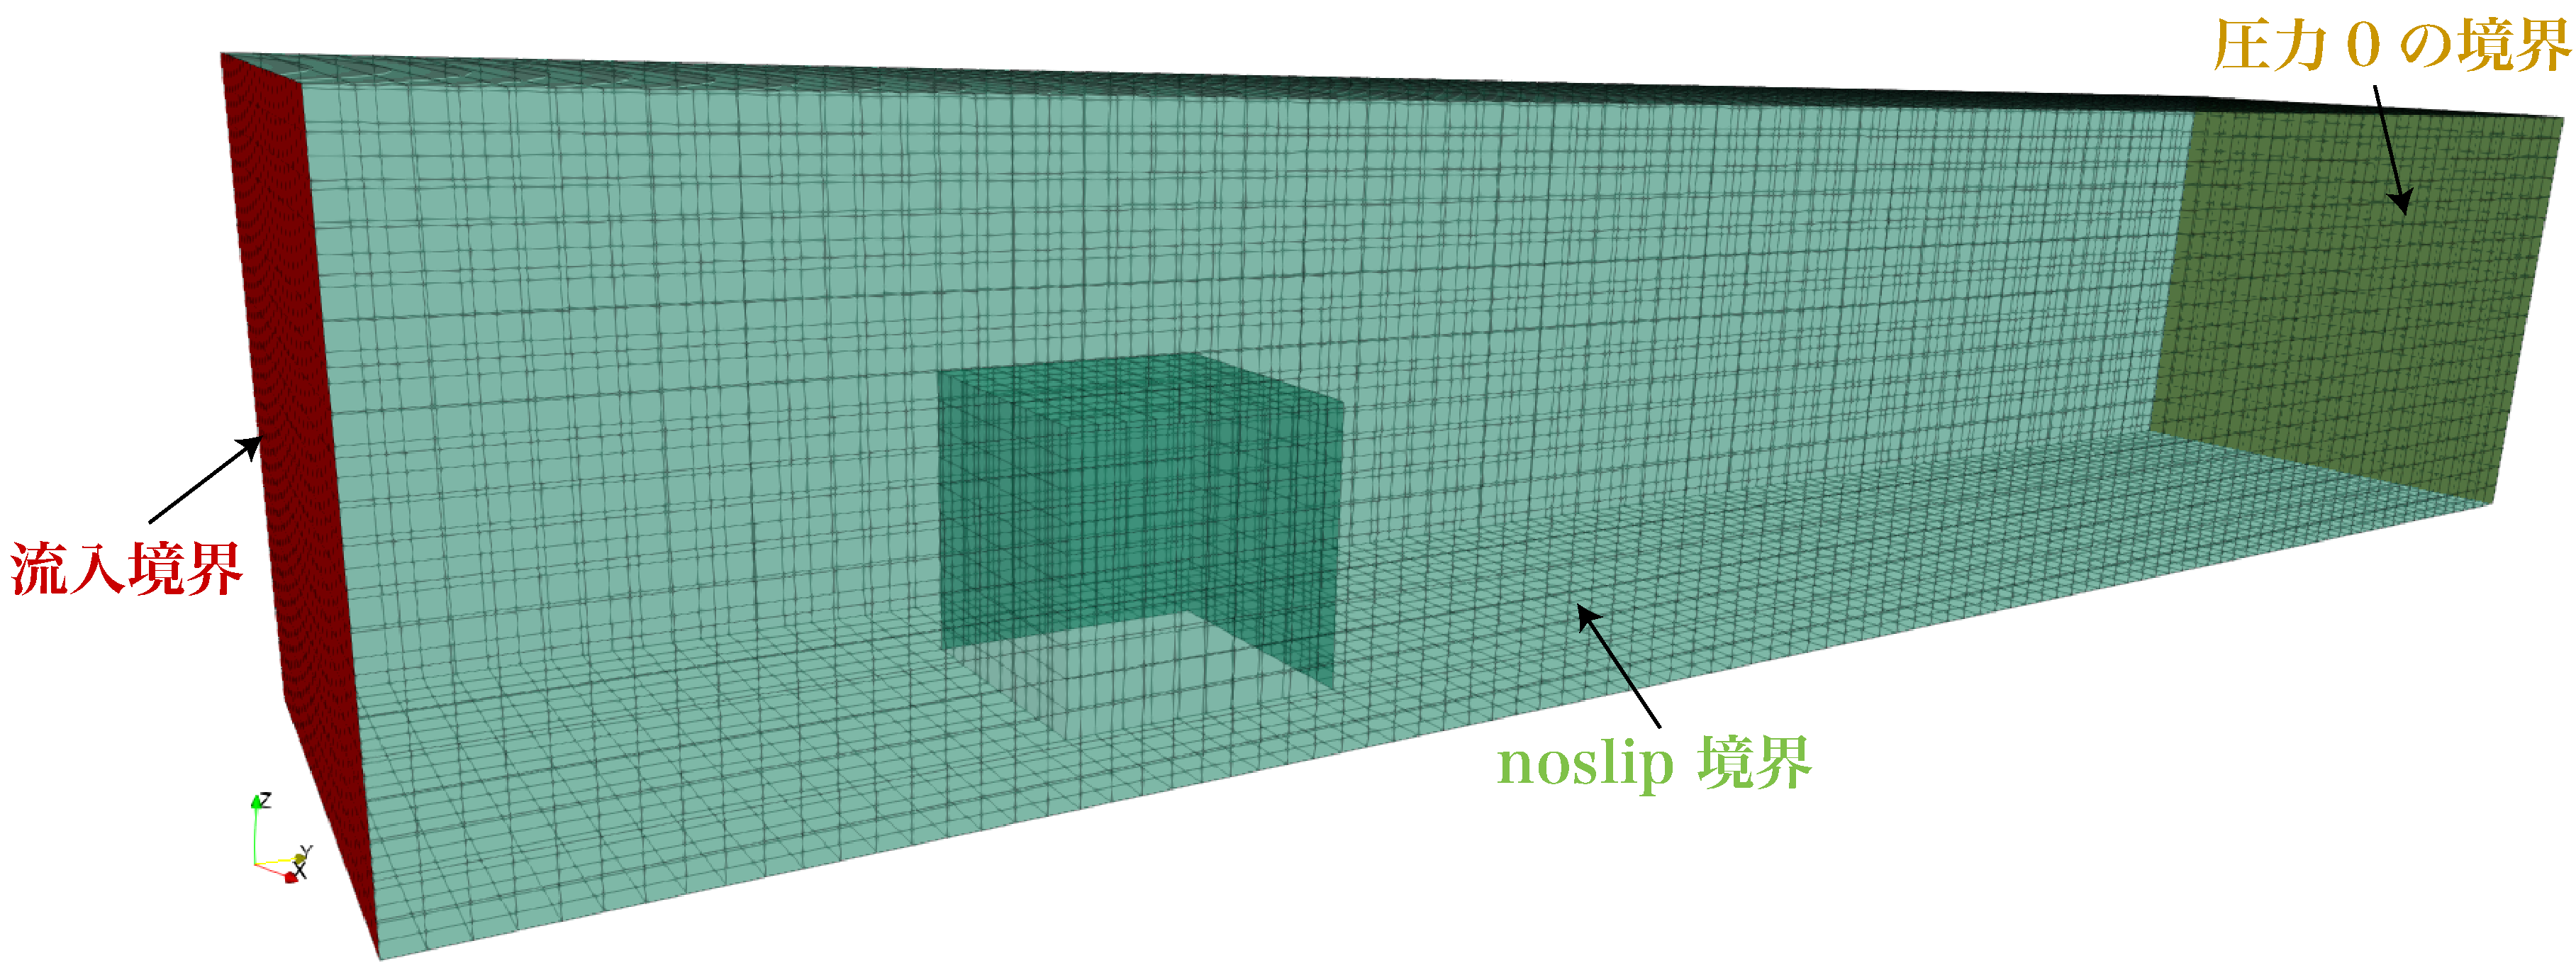
\includegraphics[width=17.2truecm]{pics/sample.pdf}
	\caption{出力された設定}
	\label{fig:schema_gcb}
\end{figure}

ソルバーに対する初期条件の指定には、以下のファイルが使用されます。
\begin{itemize}
	\item 節点および要素データ: node.dat, elem.dat
	\item 圧力の Dirichlet 境界条件ファイル : D\_bc\_p.dat
	\item 速度の Dirichlet 境界条件ファイル (流入境界条件および noslip 境界条件): D\_bc\_v.dat
\end{itemize}


%\begin{thebibliography}{99}
	%\bibitem{hughes1989new} Hughes, T.J.R., Franca, L.P., Hulbert, G.M: A new finite element formulation for CFD: VIII. The Galerkin-least-squares method for advective-diffusive equations. Computational Methods in Applied Mechanics and Engineering, 73, 173--189, 1989.
%\end{thebibliography}
\end{document}

